\documentclass[../main.tex]{subfiles}

\begin{document}

\section{Spectral pollution in a multiplication operator}
\subsection{The spectrum of a multiplication operator}
\begin{definition}{\textbf{(Multiplication operator)}}\index{operator!multiplication}
Let $\Omega$ be a $\sigma$-finite measure space.
For a given function $a$, the multiplication operator $M_a$ on $L^2(\Omega)$ is defined by
the action $M_af(x) = a(x)f(x)$; that is, it acts by pointwise multiplication with $a$. We call $a$ the `symbol' of
the multiplication operator.
\end{definition}

The spectrum of a multiplcation operator is easy to calculate. We first
need to define the 'essential range' of a function. Intuitively, this is
similar to the standard range of a function, but ignoring values taken by
the function on a set of measure zero - two functions which are equal
almost everywhere will have the same essential range.

\begin{definition}{\textbf{(Essential range and essential supremum)}}\label{defn:essential-range}\index{range!essential}
  The essential range of a real-valued function $f$ is the set:
  $$\{k \in \mathbb{R} : \forall \varepsilon > 0, \mu\{x : |f(x) - k| < \varepsilon\} > 0\}$$
  where $\mu$ is the Lebesgue measure.
  
  The essential supremum of $f$, denoted $\mathrm{esssup}f$, is the supremum of the essential range of $f$. 
  We define $\mathrm{essinf}f$ mutatis mutandis for the infimum.
\end{definition}

The normed vector space $L^\infty$ is the space of all bounded measurable functions, and its norm is $$\|f\|_\infty = \text{esssup}(|f|).$$

\begin{lemma}\label{thm:mult-symbol-char}
(Adapted from \cite{arveson2002short})
A multiplication operator is bounded if and only if its symbol is in $L^\infty$.
\end{lemma}
\begin{proof}
Let $M_a$ be a multiplication operator on a Hilbert space $H$ with symbol $a \in L^\infty$. We see that $|f(z)| \leq \|a\|_\infty$ for almost all $z$, so $|a g| = |a||g| \leq \|a\|_\infty |g|$ pointwise almost everywhere; thus
\begin{equation*}
\|a g\|_2 = \sqrt{\int |a g|^2} \leq \sqrt{\int \|a\|_\infty^2|g|^2} = \|a\|_\infty \sqrt{\int |g|^2} = \|a\|_\infty \|g\|_2. .\tag{$\star$}
\end{equation*}
This implies $\|M_a\| = \sup_{g \in H} \|a g\|_2 \leq \|a\|_\infty$, so $M_a$ is bounded.

Conversely, assume $M_a$ is bounded, $a \neq 0$ and let $c < \|a\|_\infty$ (of course, we do not assume $\|a\|_\infty$ is finite). Then we know that the
set $\{z : |a(x) > c|\}$ must have positive measure, and by $\sigma$-finiteness we have a subset $E \subseteq \{z : |a(x) > c|\}$, and its characteristic 
function $\1_E$ is in $L^2$. Then $|a \1_E| \geq c \1_E$, and by a similar calculation to ($\star$) and taking the supremum, $\|M_a  \1_E\|_2 \geq c \|\1_E\|_2$, so $\|M_a\| \geq c$. Taking the supremum over all $c$ gives $\|M_a\| \geq \|a\|_\infty$, so $\|a\|_\infty$ is finite and so $a \in L^\infty$.
\end{proof}

Note from this lemma we also get that $\|M_a\| = \|a\|_\infty$.

\begin{theorem}\label{thm:mult-op-spec}
  The spectrum of the multiplication operator $M_a$ is the essential range of its symbol $a$.
\end{theorem}
\begin{proof}
(Adapted from \cite{garcia2023operator})
Let $(M_a - \lambda)f = g$. Then $f(z) = \frac{g}{a(z) - \lambda}$, and we see that $(M_a - \lambda)$ is invertible if and only if the operator
$M_{(a - \lambda)^{-1}}$ is bounded, which is the case if and only if $(a - \lambda)^{-1} \in L^\infty$ by Lemma \ref{thm:mult-symbol-char}.
This is the case exactly when $(a - \lambda) \geq \epsilon$ almost everywhere - by definition, this means that $(M_a - \lambda)$ is invertible if and
only if $\lambda$ is not in the essential range of $a$.
\end{proof}

We will now take advantage of the ability to create simply-defined operators with easy-to-calculate
spectra to observe the existence of spectral pollution.

\subsubsection{Estimating spectra computationally}
\begin{example}
Let $M_f$ be the multiplication operator on $L^2(0, 1)$ with symbol

$$
f: x \mapsto \begin{cases}
x & x < 1/2 \\
x + 1/2 & \text{otherwise.}
\end{cases}
$$
By Theorem \ref{thm:mult-op-spec}, the spectrum of $M_f$ is the set $[0, 1/2] \cup [1, 3/2]$. If our Ritz approximation works as expected, we should
see the approximation create two dense clusters of eigenvalues which approach these intervals.
\end{example}

Figure \ref{fig:mult-op-spec} shows a plot of the approximate spectrum for various Ritz matrix sizes. This approximation was done for the sequence of
truncations $T_{25n}$ for $n \in \{2, 3, ..., 20\}$ over the orthonormal basis $\phi_n(x) = \exp(2 i \pi n x)$ for $n \in \mathbb{Z}$; each truncation was
over the space $\mathrm{span}\{\exp(2 i \pi k x), k \in \mathbb{Z}, |k| < n/2\}$.

We do successfully and rather quickly get eigenvalues corresponding to our actual spectrum, but we also get a lot of other eigenvalues; some of them are 
converging to points in the spectrum, but as the approximation improves, the pollution doesn't fully dissipate.

\begin{figure}[h]
\centering
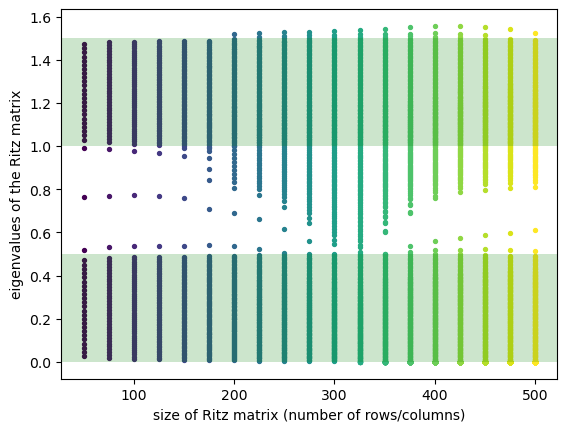
\includegraphics[scale=0.5]{mult-op-spec.png}
\caption{The approximate spectrum of the multiplication operator $M_f$ for Ritz matrices of increasing size. The shaded green areas correspond to the 
actual spectrum of the operator.}\label{fig:mult-op-spec}
\end{figure}

Some of these extra values seem to eventually converge into the correct part of the spectrum, but others stay around; in particular, for all of these approximations we have an eigenvalue of roughly 0.95 which does not exist in the operator's spectrum.

Of course, this is not particularly rigorous - we do not yet know anything about the asymptotic behaviour of the eigenvalues of these approximations (it may well converge far beyond our biggest estimate here of a $500 \times 500$ matrix) - but this example is certainly motivating. If one had no knowledge of the actual spectrum of $M_f$, they would be forgiven for considering this to be strong empirical evidence that the spectrum contains the range $[0.8, 1.0]$ or at least some subset of it. 

We have also raised a variety of other questions about the nature of this pollution - why are we only getting it in the gap between the intervals, and not far outside? Is it particular to our choice of sequence for our orthogonal projections (in particular, is there some choice which avoids pollution entirely)?

We will first discuss the nature of spectral pollution for a multiplication operator, taking advantage of an underlying structure to its Ritz matrices which 
make it possible to concretely identify the existence and location of spectral pollution. Following chapters will then devise technology that allows us to 
answer these questions in greater generality.

\subsubsection{The structure of approximations}
If we take a closer look at the structure of our approximating Ritz matrices we uncover deeper structure, which will lead
to our next topic.
\begin{example}\label{exp:mult-op-toeplitz}
Let $M_f$ be a multiplication operator on $L^2(0, 1)$. Now we create the Ritz matrix, $A_{j,k} = (M_f \phi_j, \phi_k)$, 
choosing the orthonormal basis $\phi_n(x) = \exp(2 \pi i n x).$

We now note that there is a structure to our matrix:
\begin{align*}
(M_f \phi_j, \phi_k) & = \int_0^1 f(x) \exp(2 \pi i j x) \exp(-2 \pi i k x) dx \\
& = \int_0^1 f(x) \exp(2 \pi i (j-k) x)\\
& = c_{j-k}
\end{align*}
where $c_n$ is the n'th Fourier coefficient. Thus our Ritz matrix depends only on the value of $j-k$; in particular, it is constant
along each diagonal. This is a special type of matrix known as a Toeplitz matrix.
\end{example}
As a result, the approximation of our operator $M_f$ is equal to the approximation of a infinite matrix $(T_f)_{j,k} = c_{j-k},
j,k \in \mathbb{N}_0$ by its truncations $(T_{f,n})_{j,k} = c_{j-k}$ for $j, k \leq n$. And nowhere in this derivation did we use particular
properties of $f$; we can repeat this reasoning with any function capable of being represented by a Fourier series. Let us systematise
what we have seen.

\subsection{Toeplitz operators}
\subsubsection{Toeplitz operators, Toeplitz matrices, and their equivalence}

The approximation of spectra provides a natural gateway to the study of Toeplitz operators, a type of operator with an elegant cluster
of representations that will provide intuitive and concrete insight into spectral pollution. A full account of Toeplitz theory is the subject
of whole monographs (such as \parencite{bottcher1990analysis}) and is an entire subfield in itself;
here we will stick to exploring their spectra, and how these relate to the spectra of their multiplication operator neighbours. 

\begin{definition}{\textbf{(Toeplitz matrix)}}\index{matrix!Toeplitz}
A matrix $A$ (finite or infinite) is Toeplitz if it is constant along its diagonals; that is, $A_{i,j} = A_{i+1,j+1}$
for any $i, j$ (where $i,j < N \in \mathbb{N}$ if $A$ is finite, or $i,j \in \mathbb{Z}_+$ when $A$ is infinite).
\end{definition}

Note that an infinite Toeplitz matrix induces an operator on $\ell^2(\mathbb{Z}_+)$.
We see from our example that if $f \in L^\infty$ is represented by the Fourier series
$$f(z) = \sum_{k=-\infty}^{\infty} c_k e^{i n \theta},$$
then it induces a Toeplitz matrix $T_f$ with $(T_f)_{j,k} = c_{j-k}$.
A natural question is to then ask whether a Toeplitz matrix induces a function, and the answer is affirmative. Firstly, we must define a relevant setting for our matrices; indeed, an important part of our
example was that $M_f \exp(2 \pi i j x)$ was well-defined. The following definitions are adapted from \parencite{arveson2002short}.

\begin{definition}{\textbf{(Hardy space)}}\index{Hardy space}
Let $\zeta$ be the monomial function on $L^2(\mathbb{T})$, $\zeta(z) = z$, where $\mathbb{T}$ is the unit circle. Then the
Hardy space $H^2$ is the span of all non-negative exponents of $\zeta$; $\text{span}\{1, \zeta, \zeta^2...\}$.
\end{definition}

As we are on the unit circle, $z$ is more familiarly $e^{i \theta}$ for some $\theta$; then the basis of Hardy space becomes $\{e^{i n \theta}\}_{n \in \mathbb{Z}_+}$. Then we can identify any element $f \in H^2$ as any square-integrable function defined on the unit circle with the Fourier series 
$$f(e^{i \theta}) \sim \sum_{k=0}^\infty c_k e^{i k \theta},$$

that is, with all negative Fourier coefficients equal to zero. This can be identified with the operator on $\ell^2(\mathbb{Z}+)$ via the isomorphism $\sum_{k=0}^\infty c_k e^{i k \theta} \mapsto (c_k)_{k \in \mathbb{Z}_+}$ \parencite{bottcher1990analysis}.

 A generalised definition can be made for $H^p$ via any $L^p(\mathbb{T})$; we will almost entirely use $H^2$ (with the exception of needing $H^1$ later on), which is often defined as `the' Hardy space.

\begin{definition}{\textbf{(Toeplitz operator)}}\index{operator!Toeplitz}
Let $\phi \in L^{\infty}(\mathbb{T})$ be bounded and measurable on the unit circle. The Toeplitz operator $T_\phi$ is the compression of $M_\phi$ 
to the Hardy space: $T_{\phi} = P_{H^2} M_\phi \big|_{H^2}$. We call $\phi$ the `symbol' of $T_\phi$.
\end{definition}

One may notice what appears like a clash of notation between the induced Toeplitz matrix that was just discussed with the Toeplitz operator. This is not
so; there is an elegant relation between Toeplitz operators and Toeplitz matrices.

\begin{theorem}
Let $A$ be a bounded operator on $H^2$ such that $(A \zeta^j, \zeta^k) = a_{j-k}$ for some sequence $(a_n)_{n \in \mathbb{Z}}$. Then there is
some function $\phi \in L^\infty$ such that $A = T_\phi$ and $a_n$ are the Fourier coefficients of $\phi$.
\end{theorem}
\begin{proof}
%%%%%TODO: DO WE PROVE THIS?
\end{proof}

Many properties of Toeplitz operators are hard to see via infinite matrices. Being able to represent them as both Fourier series and equally as the  
compressions of multiplication operators puts us on the firmer ground of functional analysis, rather than asymptotic linear algebra. From this, we
are now in the position to exactly calculate the spectrum of a Toeplitz operator with real-valued symbol.

\subsubsection{The spectrum of a Toeplitz operator with real symbol}

To begin, we require a pair of properties regarding functions in $L^1(\mathbb{T})$'s Hardy space, $H^1$. 

\begin{lemma}{\textbf{(Properties of $H^1$ functions)}}\label{thm:h1-properties}
Let $H^1$ be the space of all functions $f \in L^1(\mathbb{T})$ where $f$ has the Fourier series

$$f(e^{i \theta}) \sim \sum_{n=0}^\infty a_n e^{i n \theta}$$

i.e. has no negative Fourier coefficients. Then the following properties hold:
\begin{enumerate}
\item\label{item:h2-products-in-h1} If $f, g \in H^2$, then $fg \in H^1$;
\item\label{item:f-h1-const} If $f \in H^1$ is real-valued, then $f$ is constant.
\end{enumerate}
\end{lemma}
\begin{proof}
(\ref{item:h2-products-in-h1}.) Let $f, g$ be in $H^2$. Then in particular, $f, g \in L^2$, and so their product $fg$ is in $L^1$ (this can be seen directly by the H\"older inequality). Now if $f$ has Fourier coefficients $a_k$ and $g$ has Fourier coefficients $b_k$, the $k$'th Fourier coefficient of $fg$ is given by $\sum_{n \in \mathbb{Z}} a_n b_{k-n}$. For negative $k$, we now have that either $n < 0$ so $a_n = 0$, or $n \geq 0$ so $b_{k-n} = 0$ as $k-n < 0$;
this means that the Fourier series of $fg$ satisfies the Hardy space property, but we must justify that the Fourier series of a product is equal to the product of the Fourier series - indeed, they converge to $f$ in $L^2$ as 

(\ref{item:f-h1-const}.) For any real-valued function, we have the relation $\overline{c_{-n}} = c_n$ for the Fourier coefficients of $f$:
$$ \overline{c_{-n}} = \overline{\int f(x) e^{-inx} dx} = \int \overline{f(x)} e^{inx} dx = \int f(x) e^{inx} dx = c_n.$$
But if $f$ is in Hardy space, $c_{-n} = 0$ for all $n \in \mathbb{N}$, and so $c_n = \overline{c_{-n}} = 0$ for all $n \in \mathbb{N}$. Thus
the only coefficient remaining is $c_0$, and a function with a constant Fourier series is a constant function. (This proof is valid for any $H^p, p \in [1, \infty)$.)
\end{proof}

We are now in the position to calculate the form of the spectrum for any Toeplitz operator. This spectrum was first found by Toeplitz
himself under a stronger set of regularity assumptions, and then weakened by Wiener via his Tauberian theorem \parencite{schmidt1960toeplitz}.
Our proof will consist of a series of claims about the resolvent set of $T_\phi$, following a proof outlined in an exercise of Arveson (\parencite{arveson2002short}, Chapter 4.6, exercises 2-5) which is based on a proof by Hartman and Wintner.

\begin{theorem}{\textbf{(Hartman-Wintner)}}\index{theorem!Hartman-Wintner}\label{thm:hartman-wintner}
Let $\phi \in L^\infty$ be real-valued. Then $\Spec(T_\phi) = [m, M]$, where $m$ and $M$ are the infimum and supremum of the essential range of $\phi$ (Definition \ref{defn:essential-range}) respectively.
\end{theorem}
\begin{proof}
Note we already know that as $\phi$ is real-valued, $T_\phi$ is self-adjoint, and so its spectrum is on the real line. 
Furthermore, we will assume that $\phi$ is non-constant, as if $\phi$ is constant then $T_\phi$ is some constant multiple of the identity operator
and its spectrum is simply the set containing that constant, and the result holds.
\begin{enumerate}[I.]
\item Let $\lambda \in \mathbb{R}$ be such that $T_\phi - \lambda$ is invertible. Then there is a non-zero function $f \in H^2$ such that $(T_\phi - \lambda)f(z) = k$ for any $z$. By the definition of invertibility this is true for $f$ = $(T_\phi - \lambda)^{-1}\kappa$, where
$\kappa$ is the constant function in $H^2$; $\kappa : z \mapsto k$ for some $k \in \mathbb{C}.$

\item Now we claim that $(\phi - \lambda)|f|^2$ is constant almost everywhere. To do this, we first show that it is in $H^1$. Indeed, we have
$(\phi - \lambda)|f|^2 = ((\phi - \lambda)\overline{f}) f$. Then by the previous part, $$(\phi - \lambda)\overline{f} = \overline{(\phi - \lambda)f} = \overline{\kappa}$$
where $\overline{\kappa}$ maps $z$ to $\overline{k}$. Then it is still a constant function so is still in $H^2$, and by Lemma \ref{thm:h1-properties}.\ref{item:h2-products-in-h1}, $((\phi - \lambda)\overline{f}) f$ is in $H^1$ as a product of two $H^2$ functions. Now we use Lemma \ref{thm:h1-properties}.\ref{item:f-h1-const}: because $\phi$ and $\lambda$ are real-valued, $(\phi - \lambda)|f|^2$ is also real-valued, so must be constant. Let this constant be called $c$.
\item Our next claim is that $\phi - \lambda$ crosses the $x$-axis almost nowhere. This is almost immediate once we invoke a theorem of F. and M. Riesz\footnote{Which can be proven as a corollary of a famous theorem of Buerling; see \parencite{arveson2002short}, chapter 4.5.}, which states
\begin{displayquote}
\emph{Let $f$ be a non-zero function in $H^2$. Then the set $\{z \in \mathbb{T} : f(z) = 0\}$ has Lebesgue measure zero.}
\end{displayquote}
This means that $(\phi(z) - \lambda) = \frac{c}{|f(z)|^2}$ is well-defined on $L^\infty$. Then because $|f|^2 > 0$ a.e., $(\phi - \lambda)$ is positive almost everywhere if $c > 0$, and negative almost everywhere if $c < 0$. Note that if $c = 0$, then $(\phi(z) - \lambda) = 0$, so $\phi$ is the 
constant function with value $\lambda$ and the result holds by our remark at the beginning of this proof.
\item Finally, we show $\Spec(T_\phi) = [m, M]$. By our previous claim, if $T_\phi - \lambda$ is invertible, then either:
\begin{itemize}
\item $\phi(z) - \lambda < 0$ a.e., so $\phi(z) < \lambda$ a.e., so $\lambda > M$, or
\item $\phi(z) - \lambda > 0$ a.e., so by the same argument $\lambda < m$.
\end{itemize}
Thus $T_\phi - \lambda$ is invertible only outside of the set $[m, M]$, as required.
\end{enumerate}
\end{proof}

\subsubsection{Multiplication operators, Toeplitz operators, and spectral pollution}
Let us now bring the discussion back to spectral pollution, and to our discovery in Example \ref{exp:mult-op-toeplitz}. The Ritz matrices corresponding to the
multiplication operator $M_f$ is \emph{identical} to the Ritz matrices corresponding to the Toeplitz operator $T_f$ (which are just truncations of the 
corresponding Toeplitz matrix), but these operators have different spectra. No wonder we are seeing extra eigenvalues in the gap; the approximation
`cannot tell' the difference between an operator which has the essential range as its spectrum from one which has the same maximum and minimum but with
all gaps filled in. Heuristically, one may even expect that with a large enough approximation, the \emph{entire gap} could fill up with spurious
eigenvalues\footnote{We also have the inverse question; if we are approximating the Toeplitz operator $T_f$, why does it take so much longer to 
approximate the spectrum in the interval $\Spec(T_f) \setminus \Spec(M_f)$?}.\\

More rigorously, it is possible to show that for any point in a gap of the multiplication operator's spectrum, some subsequence of truncations will have 
an approximate eigenvalue converging to that point. 

\begin{theorem}{\textbf{(Schmidt-Spitzer \parencite{schmidt1960toeplitz})}}\index{theorem!Schmidt-Spitzer}
Let $T_n$ be the $n \times n$ matrix created by taking the first $n$ rows and columns of a Toeplitz operator $T_f$. Consider the set
$$B = \{\lambda \in \mathbb{C} : \lambda = \lim_{m \rightarrow \infty} \lambda_{i_m}, \lambda_{i_m} \in \Spec(T_{i_m}), i_m \rightarrow \infty \}.$$
where $i_m$ is a subsequence of $\mathbb{N}$. Then if $f$ is real-valued, $B = \Spec(T_f)$.
\end{theorem}
\begin{proof}
If $f$ is real-valued, then the corresponding Toeplitz matrix is Hermitian; its Fourier coefficients have the property $\overline{c_{-n}} = c_n$ (see 
the proof of Lemma \ref{thm:h1-properties}.\ref{item:f-h1-const}), so if $A$ is the corresponding Toeplitz matrix,
 $A_{i,j} = c_{i-j} = \overline{c_{j-i}} = \overline{A_{j,i}}$. Label the eigenvalues of $T_n$ as $\lambda_{n_1}, ... \lambda_{n_{n+1}}$. 
 
 We now invoke a theorem of Szeg\"o \cite{grenander2001toeplitz} regarding the distribution of eigenvalues: on any real interval $[a, b]$,
\begin{equation}\label{eqn:szego-eigvals}
\lim_{n \rightarrow \infty} \frac{1}{n+1} \sum_{i=1}^{n+1} \1_{[a, b]}(\lambda_{n_i}) = \frac{1}{2 \pi} \mu\{\theta : a \leq f(e^{i \theta}) \leq b\}
\end{equation}
where $\mu$ is the Lebesgue measure, and $\1$ the characteristic function of $[a,b]$ 
(i.e. $\1_{[a, b]}(\lambda_{n_i})$ is 1 if $\lambda_{n_i} \in [a, b]$ and zero otherwise). Note that this makes sense, as $T_n$ is Hermitian and
therefore every eigenvalue is real-valued. Note also that by Theorem \ref{thm:hartman-wintner} and the definition of the unit circle $\mathbb{T}$,
the spectrum of $T_f$ is $\{f(e^{i \theta}): \theta \in [0, 2\pi]\}$. The claim of equation (\ref{eqn:szego-eigvals}) is therefore 
``as the size of the Toeplitz matrix increases, the proportion of eigenvalues of $T_n$ in $[a, b]$ converges to the proportion of the spectrum in $[a, b]$''. 
Of course, this proportion will never be 0 for any interval $[a, b] \subseteq [\textrm{essinf}f, \textrm{esssup}f]$ of positive measure, so we can guarantee that a sequence of truncations has an eigenvalue which converges in $[a, b]$. The result follows.

\end{proof}

This is a striking result - for any point in the spectral gap $\Spec(T_f) \setminus \Spec(M_f)$ (or indeed in $\Spec(M_f)$, but they aren't really polluting anything), we can choose a sequence of truncations such that
there is guaranteed to be spectral pollution at that point!

\end{document}
